%% Methodology
%%=========================================

\chapter{Methodology}
\label{ch:methodology}
This chapter presents the research methodology that was used in the process of writing this master thesis. The chapter looks closer at the research questions and how these were used as premise for how the research was conducted. In addition, the chapter explains our general research strategy.

%%=========================================

\section{Evaluating Research Questions}
\label{sec:research_questions_and_approach}
To recap from section \ref{sec:goals_and_research_questions}, we presented our research questions as:

\begin{description}
    \item[Research Question 1]{\textit{Does ambiguity in character signature sequences impact recognition rates?}}
    \item[Research Question 2]{\textit{Does different fonts, font characteristics, font styles, and other typesetting factors affect recognition rates?}}
    \item[Research Question 3]{\textit{Can a signature sequence based model handle multiple fonts at the same time?}}
\end{description}

Concerning \textbf{RQ1}, we knew ambiguity could be a problem for the general problem we were trying to solve. This was made clear early in testing and is expanded on further in section \ref{sec:ambiguous_input}. To answer this research question we would need to conduct tests and experiments where we compare sequences with and without ambiguities to see how the differences impact the recognition rates.

Answering \textbf{RQ2} could also be done in similar fashion as the previous research question. Running multiple tests with different combinations of fonts, their characteristics, styles etc would give answer to just how much recognition rates were affected. These factors are explained more in detail in sections \ref{sec:tuning_input_data}, \ref{sec:use_of_fonts}, and \ref{sec:other_factors}.

Finally, answering \textbf{RQ3} would also require running a series of tests and experiments to see how the rates are affected.

%%=========================================

\section{Research Approaches}
Figure \ref{fig:model_research_process} contains the model of the research process, as presented in \citep{oates2005researching}. The figure displays the steps in a research process from start to finish. It illustrates how various approaches can be used, and how it is also possible to mix and combine strategies and data generation methods.

\begin{figure}[ht]
    \centering
    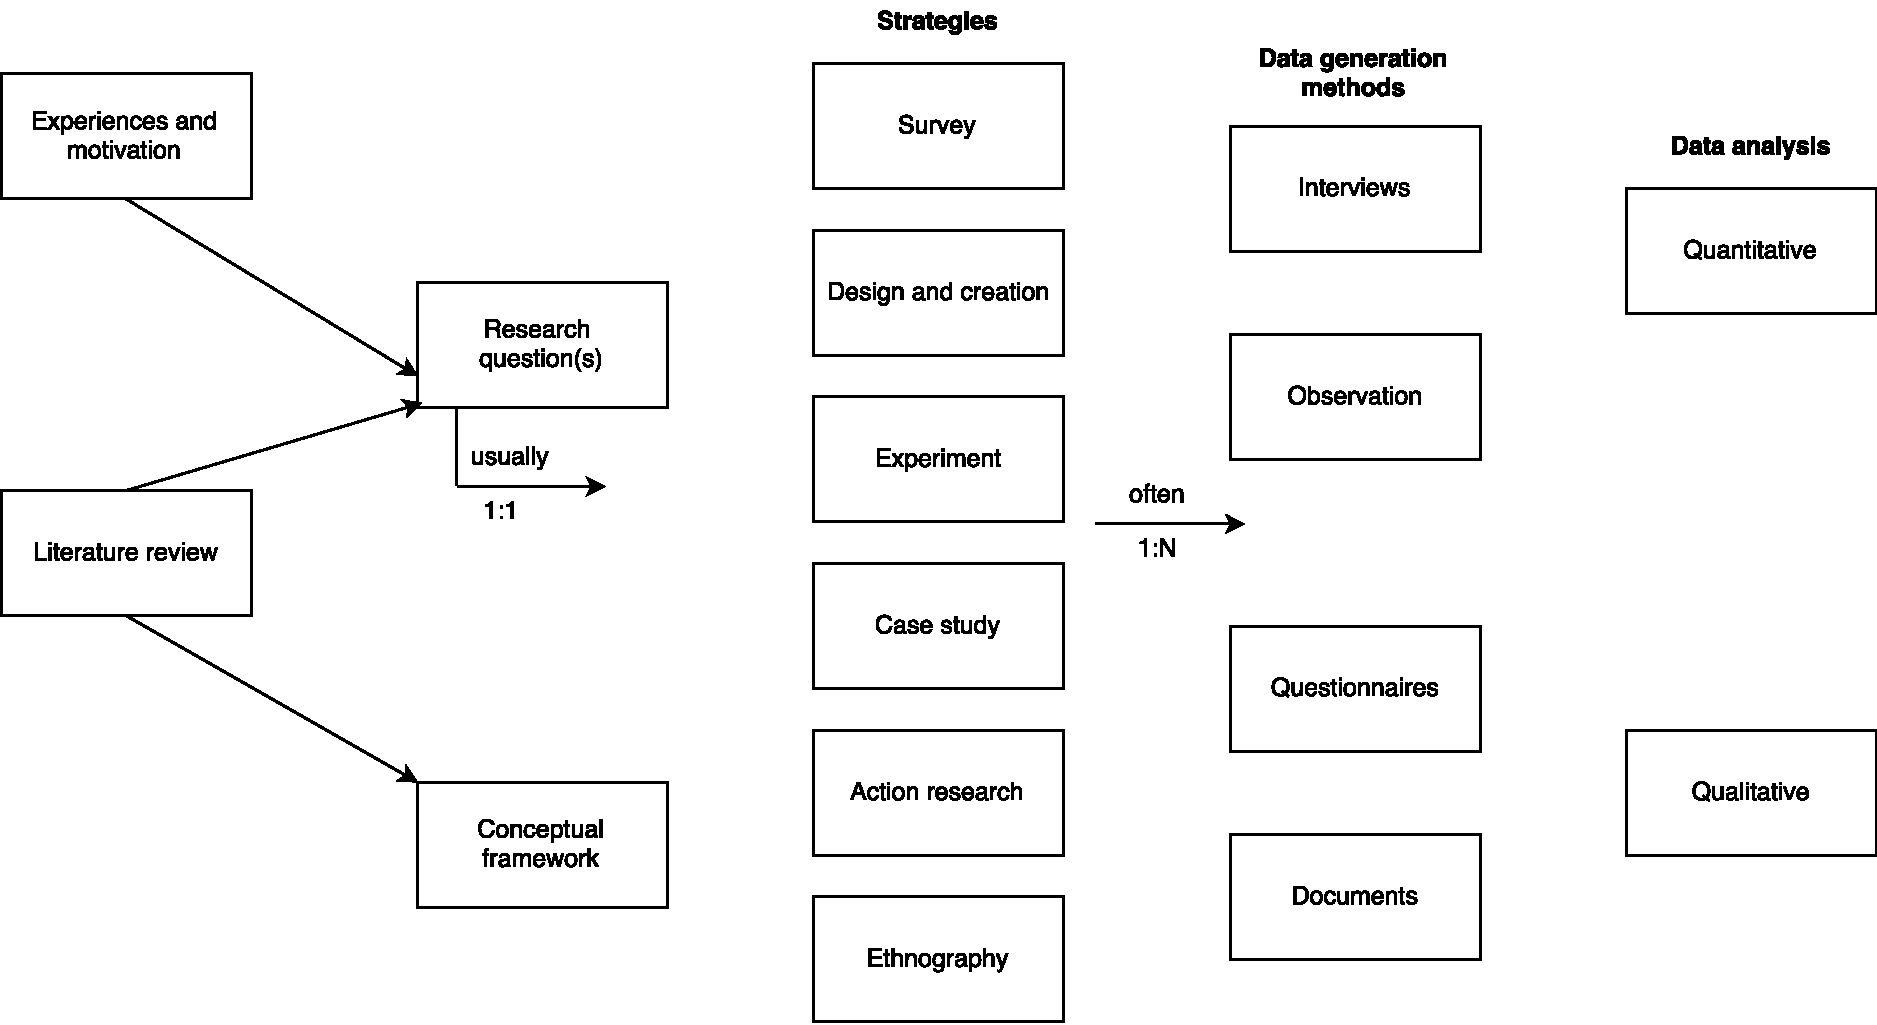
\includegraphics[width=0.9\textwidth]{fig/methodology/research_strategies.pdf}
    \caption{Model of the research process}
    \label{fig:model_research_process}
\end{figure}

The literature review is presented in Chapter \ref{ch:related_work}. The research questions was presented in section \ref{sec:goals_and_research_questions}, and was expanded on further in section \ref{sec:research_questions_and_approach}. The conceptual framework is what is presented throughout this chapter. Our choice of research strategy is presented in section \ref{sec:research_strategy}. Our choice of data generation methods, as well as our data analysis approach is presented in section \ref{sec:data_generation_methods_and_data_analysis}.

%%=========================================

\section{Research Strategy}
\label{sec:research_strategy}
The research strategy used in this master thesis was carefully chosen on the premise of what our research questions and what our overarching research goal were. As stated in section \ref{sec:research_questions_and_approach}, our argument is that the research questions could be answered by conducting experiments and tests. This fact was used as the foundation for the research strategy that was used throughout the work on this master thesis.

Our choice of the overarching research strategies were design and creation combined with experiments. As illustrated in Figure \ref{fig:model_research_process}, it is most common to use a single research strategy, but it is also possible to combine them in the research. Our combination of research strategies allowed us to iteratively build a model, testing various approaches to find an optimal solution. We followed the strategy of design and creation for the most part, but paid close attention as to why we got the results we got during the development process. While the strategy of design and creation is built on the concept of iteratively building a product, experiments is a strategy that investigates cause and effect relationships. We used experiments and the investigations to help us steer the development in the correct course, by investigating the current results.

In \ref{sec:design_and_creation} and \ref{sec:experiment} we present the research approaches of design and creation and experiments in greater depth. In \ref{sec:combining_the_two_strategies} we elaborate on how we combined the two research strategies together in our process.

%%=========================================

\section{Design and Creation}
\label{sec:design_and_creation}
Development of a new IT product is the main focus of the design and creation research strategy. IT products are also called artefacts, and there are four of these. These are \citep{march1995design, oates2005researching}:

\begin{itemize}
    \item\textbf{Constructs:} the concepts or vocabulary used in a particular IT-related domain. For example, notions of entities, objects or data flows.
    \item\textbf{Models:} combinations of constructs that represent a situation and are used to aid problem understanding and solution development. For example, a data flow diagram, a use case scenario or a storyboard.
    \item\textbf{Methods:} guidance on the models to be produced and process stages to be followed to solve problems using IT. For example, formal, mathematical algorithms, or commercialized and published methodologies.
    \item\textbf{Instantiantions:} a working system that demonstrates that constructs, models, methods, ideas, genres or theories can be implemented in a computer-based system.
\end{itemize}

In our case, the artefact we want to develop during our research would fall into the category of instantiantions. This artefact would be a fully functional system that works on the premise of our research.  As this system would be an essential part of the research process, it is important that it can be considered as research, and not just as a demonstration of technical powers. It is therefore essential that the system is not only developed, but the process also assert the academical qualities, such as analysis, explanation, argument, justification, and critical evaluation \citep{oates2005researching}. This means that every part of our system, and the process of building it, is explained and reasoned.

\subsection{Approach}
\label{methodology-design-and-creation-approach}
The approach in design and creation revolves around a problem-solving strategy. It utilizes an iterative process over five steps \citep{vaishnavi2004design, oates2005researching}:

\begin{itemize}
    \item\textbf{Awareness:} involves recognizing a problem. This step is necessary to find what problem we are trying to solve.
    \item\textbf{Suggestion:} is the step where we create a tentative idea of how the problem might be addressed.
    \item\textbf{Development:} is where we implement and idea from the previous step.
    \item\textbf{Evaluation:} involves examine the artefact and evaluations are done to estimate its worth and deviations from the expectations.
    \item\textbf{Conclusion:} is the final step in the cycle where results are collected and written down. Gained knowledge is identified and any unexpected or unexplainable results could lay the ground for further research.
\end{itemize}

It is important to understand that these steps are not necessarily followed in a strict manner. Instead, they work as guidelines, and the process is more of a fluid iterative cycle where the approach may shift depending on problem or situation. \citep{oates2005researching} explains how these cycles work and what you as a researcher achieves by using this research method as follows:

\begin{quote}
    Thinking about a suggested tentative solution leads to greater awareness of the nature of the problem; development of a design idea leads to increased understating of the problem and new, alternative tentative solution; discovering that a design doesn't work according to the researcher's expectations leads to new insights and theories about the nature of the problem, and so on. 
\end{quote}

The goal is to work out a prototype that is gradually modified until a satisfactory implementation is produced. One of the biggest advantages of this approach is that it is not necessary to fully understand a problem before developing prototypes and exploring tentative solutions. This research strategy also opens up the possibilities of testing prototypes often and comparing results along the way to see if one direction or approach works better than others. As an essential part of this strategy, it must be made clear how the implemented solution emerged as a result of the repeated cycles. Without a thought-through design rationale, the final implementation may appear to be the result of a hacked together solution without any recollection of the trial and error phase.

\subsection{Evaluation and Gained Experience}
\label{sec:evaluation_and_gained_experience}
One important aspect of the process is the step of evaluation. It is very important to evaluate our prototype as the process is ongoing. There are many types of criteria that may be applied to a prototype such as functionally, completeness, consistency, accuracy, performance, reliability, usability, accessibility, and so on. Creating a classifier system, we want to focus mainly on accuracy, and valuate how well it can classify a set of problems. In addition to this measure, we also want to investigate the results and attempt to unveil why we got the results we got. If the system performs poorly, why is that? Is there something fundamentally wrong with our approach? Is our model designed in a way that is not fit with the data we are feeding it? Evaluation is critical in the step of ``learning from our mistakes". It is difficult to succeed right away, especially with lack of knowledge. Evaluating and understanding what we need to change is one of the most fundamental steps in the process of design and creation as a research strategy.

%%=========================================

\section{Experiment}
\label{sec:experiment}
Experiments are, as already mentioned, a research strategy that focuses on investigating cause and effect, and the reason between the two. During our process, this strategy helped us find out in what direction we should look to improve our model.

Experiments are structured around hypothesis. With a given hypothesis, an experiment is designed to prove or disprove the hypothesis. For example, a hypothesis may be:

\begin{description}
    \item[Hypothesis:]{\textit{if I go outside in the rain I am going to get wet.}}
\end{description}

According to \citep{oates2005researching}, research strategies that are based on experiments may, among others, be characterized by:

\begin{itemize}
    \item Observation and measurement. Here the researchers make precise and detailed observation of outcomes and changes that occur when a particular factor is introduced.
    \item Proving or disproving a relationship between two or more factors.
    \item Explanation and prediction. The researchers are able to explain the casual link between two factors.
    \item Repetition, where experiments are carried out multiple times. This is done under varying conditions, to be certain that the observed and measured outcomes are not caused by some other factor.
\end{itemize}

One of the prime focuses for our experiments were to have good internal validity. This means that measurements are obtained are cause and effect from manipulations of the independent variable, and not to any other factors. Running tests on our system this meant that we made sure to run tests on same data sets, and avoided to do any alterations except the ones we were measuring to answer our hypothesis.

%%=========================================

\section{Combining the Two Strategies}
\label{sec:combining_the_two_strategies}
As stated earlier, we did not use both of the strategies in its complete form throughout the entire process. Instead we lent on the fluid nature of design and creation, and used concepts from experiments to help us move forward. 

We created meaningful hypothesis related to the current tentative solution for a problem. While implementing the solution, we also made sure to construct it in such a way that we could test our hypothesis when it was finished. We evaluated the results from the development process, and cross examine them with the results from the investigation of our hypothesis. The combined knowledge gained though this approach helped us in the next cycle of development by uncovering which ``rock" to look under next.

%%=========================================

\section{Data Generation Methods and Data Analysis}
\label{sec:data_generation_methods_and_data_analysis}
Data generation methods is the means by which we produce the empirical data on which we evaluate our research. As state by \citep{oates2005researching}, many researchers who choose to use the design and creation strategy pay little attention to using properly the various data generation methods. Reason for this may be because the artefact that is developed needs to be tested in a specific way. In our case we wish to create a system. Evaluation of a system like this is usually done by training and testing it. Such data generation methods falls outside the regular approach as presented in Figure \ref{fig:model_research_process}.

Data analysis based on the data from our tests will be done quantitatively. This means that our data and evidence is based on numbers. The data will be compared, and analysed using tables, charts and graphs. Developing a iterative system like we are doing, this type of analysis would make it easier to compare numbers, behavior and progression.